\documentclass[11pt]{article}
\usepackage[T1]{fontenc}
\usepackage[utf8]{inputenc}
\DeclareUnicodeCharacter{00A0}{~}
\usepackage{lmodern}
\usepackage[swissgerman]{babel}
\usepackage{microtype}

\usepackage{graphicx}
\usepackage[hypertexnames=false]{hyperref}
\usepackage{xurl}
\usepackage{xcolor}
\usepackage{pdflscape}

\usepackage{tikz}
\usetikzlibrary{arrows.meta,positioning}
\usetikzlibrary{calc,chains,shapes,fit}

\graphicspath{{diagrams/}}
\usepackage{float}

\usepackage{array}
\usepackage{ragged2e}
\usepackage{tabularx}
\usepackage{longtable}
\usepackage{ltablex}
\keepXColumns

\usepackage{listings}

% Define custom languages for listings (YAML and NGINX)
\lstdefinelanguage{yaml}{
  keywords={true,false,null,y,n,yes,no,on,off},
  comment=[l]{\#},
  morestring=[b]',
  morestring=[b]",
  sensitive=true
}
\lstdefinelanguage{nginx}{
  keywords={server,location,listen,server\_name,root,index,proxy\_pass,include,ssl\_certificate,ssl\_certificate\_key,return,if,set,add\_header,client\_max\_body\_size,upstream,resolver,proxy\_set\_header,proxy\_redirect,expires,try\_files,access\_log,error\_log},
  comment=[l]{\#},
  morestring=[b]",
  morestring=[b]',
  sensitive=true
}

\usepackage{geometry}
\geometry{a4paper, top=20mm, left=20mm, right=20mm, bottom=25mm}

\usepackage{fancyhdr}
\setlength{\headheight}{15pt}
\pagestyle{fancy}
\lhead{Luca Güttinger}
\rhead{\today}
\rfoot{Seite \thepage}
\cfoot{}
\lfoot{\footnotesize\mbox{\url{https://github.com/Notenverwaltung-ch/Notenverwaltung}}}

\lstset{
    inputencoding=utf8,
    language=SQL,
    basicstyle=\small\ttfamily,
    breaklines=true,
    breakatwhitespace=true,
    columns=fullflexible,
    keepspaces=true,
    showstringspaces=false,
    tabsize=2,
    postbreak=\mbox{\textcolor{red}{$\hookrightarrow$}\space},
    literate={ä}{{\"a}}1 {ö}{{\"o}}1 {ü}{{\"u}}1 {Ä}{{\"A}}1 {Ö}{{\"O}}1 {Ü}{{\"U}}1 {ß}{{\ss}}1 {é}{{\'e}}1 {è}{{\`e}}1 {à}{{\`a}}1 {ê}{{\^e}}1 {ô}{{\^o}}1 {É}{{\'E}}1
}

\newcommand{\code}[1]{\texttt{\detokenize{#1}}}

\newcolumntype{L}[1]{>{\raggedright\arraybackslash}p{#1}}
\newcolumntype{C}[1]{>{\centering\arraybackslash}p{#1}}
\newcolumntype{R}[1]{>{\raggedleft\arraybackslash}p{#1}}
\newcolumntype{Y}{>{\raggedright\arraybackslash}X}

\setlength{\parindent}{0pt}
\setlength{\parskip}{6pt}

\setcounter{tocdepth}{4}
\setcounter{secnumdepth}{4}

\begin{document}

    \hypersetup{pageanchor=false}
% ---------------- Titelseite ----------------
    \begin{titlepage}
        \centering
        {\huge\bfseries Notenverwaltungssystem \par}
        \vspace{2cm}
        {\Large Luca Güttinger \par}
        \vspace{0.5cm}
        {\Large Dipl. Informatiker Applikationsentwicklung \par}
        \vspace{0.5cm}
        {\Large TEKO Zürich \par}
        \vspace{0.5cm}
        {\Large Netzwerkbetriebsysteme \par}
        {\Large Dozent: Uta Enke \par}
        \vspace{0.5cm}
        {\Large Abgabedatum: 22.09.2025 \par}
        \vfill
    \end{titlepage}
    \clearpage
    \hypersetup{pageanchor=true}
    \pagenumbering{arabic}

% ---------------- Inhaltsverzeichnis ----------------
    \tableofcontents
    \newpage


    \section{Einleitung}

    Dieses Dokument beschreibt die Bereitstellung (Deployment) der entwickelten Notenverwaltungsapplikation. Ein zentraler
    Bestandteil des Deployments ist es, die Anwendung auf der Zielumgebung zu installieren und fachgerecht einzurichten,
    sodass sie sicher, zuverlässig und performant betrieben werden kann. Dazu gehören insbesondere die Vorbereitung der
    Infrastruktur (Server, Netzwerk und DNS), das Starten der benötigten Container (Reverse Proxy, Backend-API, Frontend
    sowie optionale Tools) sowie die Konfiguration anwendungsspezifischer Einstellungen.

    \subsection{Ziel}
    Ziel dieses Dokuments ist es, Administratorinnen und Administratoren eine klare, reproduzierbare Anleitung an die
    Hand zu geben, um die Notenverwaltung von der leeren Zielumgebung bis zum lauffähigen System zu bringen.
    Dabei werden Installations- und Einrichtungsschritte verständlich erklärt und mit Architekturhinweisen ergänzt.

    \subsection{Voraussetzungen}
    Für das Deployment werden grundlegende Kenntnisse im Umgang mit Docker und Docker Compose vorausgesetzt.
    Zudem werden Zugriff auf den Zielserver, die Einrichtung der DNS-Einträge (z.\,B. via Cloudflare) sowie die in diesem
    Dokument genannten Zugangsdaten und Konfigurationsdateien benötigt.


    \section{Architektur}

    \subsection{Übersicht}

    Die Notenverwaltung läuft auf einem Hetzner Cloud Server in einem gemeinsamen Docker-Netzwerk (\texttt{notenverwaltung\_productive}).
    Ein NGINX Reverse Proxy exponiert Port 80 nach aussen und leitet anhand des Hostnamens die Anfragen an die internen
    Container weiter: \code{notenverwaltung.ch} zum Angular-Frontend (intern Port 80), \code{api.notenverwaltung.ch} zur
    Spring-Boot-API (intern Port 8080) und \code{pgadmin.notenverwaltung.ch} zu pgAdmin. Die DNS-Auflösung erfolgt über Cloudflare,
    wo die A/AAAA-Records auf die Server-IP zeigen. Zusätzlich schützt eine Hetzner Cloud Firewall den Server und lässt aus
    dem Internet nur HTTP (Port 80) und HTTPS (Port 443) zu (SSH auf Port 22 für Administration).

    % Architekturdiagramm
    \begin{figure}[H]
        \centering
        \resizebox{\linewidth}{!}{
            \begin{tikzpicture}[
                every node/.style={font=\small},
                box/.style={draw, rounded corners, thick, align=center, inner sep=6pt, fill=white, text width=4.6cm},
                group/.style={draw, rounded corners, thick, align=center, inner sep=8pt, fill=gray!10},
                rel/.style={-Latex, thick},
                edgelabel/.style={font=\scriptsize, fill=white, inner sep=1pt, text=black}
            ]
                % Cloudflare DNS
                \node[box, fill=orange!20, minimum width=5.5cm, text width=5.2cm] (cloudflare) {Cloudflare DNS\\DNS Records\\\texttt{A/AAAA} -> Server IP};

                % Hetzner Cloud Server (full width)
                \node[group, below=1.8cm of cloudflare, minimum width=17.0cm, minimum height=1.0cm, anchor=north] (hetzner) {Hetzner Cloud Server};

                % Docker network group inside Hetzner (full width)
                \node[group, below=1.4cm of hetzner.south, anchor=north, minimum width=16.6cm, minimum height=10.4cm] (net) {};

                % Containers inside the Docker network (proxy on top, three services side-by-side)
                % Proxy NGINX (exposed 80) near top center
                \node[box, fill=blue!15, minimum width=5.6cm, text width=5.2cm] (proxy) at ($(net.north)!0.28!(net.south)$) {NGINX Reverse Proxy\\exposed: 80/tcp};

                % T-shape: Spring centered under proxy; Angular left; pgAdmin right with tight spacing
                \node[box, fill=teal!15, below=1.6cm of proxy, minimum width=5.0cm, text width=4.6cm] (spring) {Spring Boot API\\internal: 8080};
                \node[box, fill=green!15, left=0.4cm of spring, minimum width=5.0cm, text width=4.6cm] (angular) {Angular App\\internal: 80};
                \node[box, fill=purple!15, right=0.4cm of spring, minimum width=5.0cm, text width=4.6cm] (pgadmin) {pgAdmin\\internal: default port};

                % External access arrows to proxy (split to avoid overlap)
                \node[edgelabel, above=0.4cm of hetzner.north] (dnshttp) {HTTP 80};
                \node[edgelabel, left=0.0cm of dnshttp, xshift=-2.0cm] (host1) {notenverwaltung.ch};
                \node[edgelabel, right=0.0cm of dnshttp, xshift=2.0cm] (host2) {api.notenverwaltung.ch};
                \node[edgelabel, below=0.0cm of dnshttp] (host3) {pgadmin.notenverwaltung.ch};
                \draw[rel] (cloudflare.south) -- (hetzner.north);
                \draw[rel] (hetzner) -- (proxy);

                % Proxy routing rules: straight down to Spring; short diagonals to Angular/pgAdmin
                \draw[rel] (proxy.south) -- node[edgelabel]{api.notenverwaltung.ch:80} (spring.north);
                \draw[rel] (proxy.south west) -- node[edgelabel, left]{notenverwaltung.ch:80} (angular.north east);
                \draw[rel] (proxy.south east) -- node[edgelabel, right]{pgadmin.notenverwaltung.ch:80} (pgadmin.north west);

                % Centered container group box sized to full width appearance
                \node[draw, rounded corners, thick, minimum width=16.0cm, minimum height=8.8cm, anchor=center] (containersbox) at (net.center) {};
                \node[above=2mm of containersbox.north] {Container im Netzwerk};
                % Docker Network label moved inside the containers box (top-left corner)
                \node[anchor=north west, font=\small, align=left] at ([xshift=3mm,yshift=-3mm]containersbox.north west) {Docker Network: \texttt{notenverwaltung\_productive}};

            \end{tikzpicture}
        }
        \caption{Architekturübersicht: Reverse Proxy, Angular Frontend, Spring API und pgAdmin in Docker-Netzwerk auf Hetzner. DNS via Cloudflare.}
        \label{fig:architecture}
    \end{figure}

    \subsection{Hetzner Cloud Server}
    Es wird ein Cloud Server bei Hetzner verwendet. Der Server hat folgende Spezifikationen:
    \begin{itemize}
        \item Name: CPX21
        \item 4 GB RAM
        \item 80 GB SSD
        \item 20 TB Traffic
        \item Ubuntu 24.04 LTS
        \item 3 vCPUs (AMD EPYC 7002 Series)
        \item 1 IPv4 Adresse
    \end{itemize}

    Zusätzlich wird ein Volume mit 20 GB Speicherplatz hinzugefügt, damit die Daten der Datenbank persistent gespeichert werden.

    \subsection{Cloudflare}
    Cloudflare übernimmt die DNS-Auflösung für alle öffentlichen Hostnamen. Folgende Records sind erforderlich:
    \begin{itemize}
        \item A/AAAA für \code{notenverwaltung.ch} auf die öffentliche IP des Hetzner-Servers (Proxied).
        \item A/AAAA für \code{api.notenverwaltung.ch} auf dieselbe IP (Proxied).
        \item A/AAAA für \code{pgadmin.notenverwaltung.ch} auf dieselbe IP (Proxied).
    \end{itemize}
    Zudem wird in Cloudflare HTTPS erzwungen: Aktivieren Sie unter SSL/TLS die Option \emph{Always Use HTTPS} (und optional \emph{Automatic HTTPS Rewrites}).

    \subsection{Docker Netzwerk}
    Die Container laufen in einem dedizierten Docker-Netzwerk \code{notenverwaltung\_productive}. Dieses Netzwerk isoliert
    die Dienste vom Host und erlaubt eine Namensauflösung zwischen den Containern. Nur der Reverse Proxy exponiert Ports nach aussen.

    \subsection{NGINX Reverse Proxy}
    Der Reverse Proxy lauscht extern auf Port 80 und routet anhand des Host-Headers:
    \begin{itemize}
        \item notenverwaltung.ch -> Angular-Container (intern Port 80)
        \item api.notenverwaltung.ch -> Spring Boot API (intern Port 8080)
        \item pgadmin.notenverwaltung.ch -> pgAdmin (interner Standardport)
    \end{itemize}
    Er dient als zentrale Eintrittsstelle, kann statische Inhalte des Frontends ausliefern und setzt bei Bedarf Sicherheitsheader.

    \subsection{Angular App}
    Das Angular-Frontend wird als Container betrieben und ist im internen Netzwerk unter Port 80 erreichbar.
    Der Zugriff von aussen erfolgt ausschliesslich über den Reverse Proxy und den Hostnamen \code{notenverwaltung.ch}.
    Build-spezifische Einstellungen (API-URL) werden im Image bzw. in der NGINX-Frontend-Konfiguration hinterlegt.

    \subsection{Spring Boot API}
    Die Spring-Boot-Applikation stellt die REST-API auf Port 8080 (intern) bereit. Sie ist nicht direkt von aussen erreichbar;
    Zugriffe erfolgen ausschliesslich über den Reverse Proxy unter \code{api.notenverwaltung.ch}.
    Konfigurationen (z. B. Profile, Datenbank-URL, Credentials) werden über \code{application.yml} bzw. Umgebungsvariablen gesetzt.

    \subsection{pgAdmin}
    pgAdmin dient der administrativen Verwaltung der PostgreSQL-Datenbank und ist intern auf dem Standardport verfügbar.
    Der externe Zugriff erfolgt optional über den Reverse Proxy und den Hostnamen \code{pgadmin.notenverwaltung.ch}.
    Der Zugang wird mithilfe von Benutzername und Passwort geschützt.


    \section{Deployment}

    \subsection{Github Actions}
    Die CI/CD-Pipeline ist in GitHub Actions definiert (siehe \code{.github/workflows/version-build.yml}). Bei jedem \emph{push} wird:
    \begin{enumerate}
        \item die Version ermittelt und als Tag erzeugt (Basis aus \code{build.gradle.kts}, Patch automatisch aus bestehenden Tags),
        \item das Projekt mit Gradle gebaut (Java 17, Temurin), Tests werden ausgeführt,
        \item das erzeugte Artefakt \code{build/libs/app.jar} in \code{app.jar} umbenannt und als Workflow-Artefakt abgelegt,
        \item optional ein Docker-Image gebaut und für das Runtime-Deployment bereitgestellt.
    \end{enumerate}
    Die Versionierung verwendet das Schema \code{X.Y.Z} (bzw. \code{X.Y.Z-<shortSha>} auf Feature-Branches). Auf dem \code{master}-Branch
    werden reine Release-Tags ohne Suffix erstellt.

    \subsection{Spring Applikation}
    Die Spring-Boot-Applikation wird als einzelnes Jar (\code{app.jar}) gebaut und in einem minimalen Container
    (Temurin JRE 17, Alpine)betrieben, siehe \code{Dockerfile}.\newline
    Wichtige Eckpunkte:
    \begin{itemize}
        \item Exponierter Container-Port: \code{8080} (intern; extern nur via Reverse Proxy erreichbar).
        \item Konfiguration über \code{application.yml} und Umgebungsvariablen (z. B. \code{DB_URL}, \code{DB_USERNAME}, \code{DB_PASSWORD}, \code{JWT_SECRET}).
        \item Flyway-Migrationen werden beim Start ausgeführt (\code{spring.flyway.enabled=true}).
        \item Logging ist auf INFO konfiguriert; Swagger UI ist unter \code{/public/docs} verfügbar (nur hinter dem Proxy exponiert).
    \end{itemize}
    Die Datenbankverbindung referenziert standardmässig den Hostnamen \code{postgres} im Docker-Netz. In der Produktivumgebung wird die URL über \code{DB_URL} gesetzt.

    \subsection{Angular Frontend}
    Das Angular-Frontend wird separat gebaut (\code{ng build --configuration=production}) und als statische Web-App ausgeliefert.
    Für den Produktivbetrieb wird es in einem NGINX-Container betrieben und über den Reverse Proxy unter \code{https://notenverwaltung.ch} veröffentlicht.\newline
    Die API-Basis-URL zeigt auf \code{https://api.notenverwaltung.ch}. Build-spezifische Einstellungen werden während
    des CI-Builds bzw. im NGINX-Site-Template gesetzt.

    \subsection{Release}
    Releases entstehen automatisch, wenn Commits auf \code{master} gepusht werden: Die Pipeline vergibt einen neuen Tag (\code{X.Y.Z}),
    baut Backend und Frontend und veröffentlicht die Artefakte (Jar und ggf. Docker-Image). Für manuelle Releases kann ein
    Tag ebenfalls direkt erstellt werden; die Pipeline verwendet dann exakt diesen Tag.\newline
    Der Rollout auf den Server erfolgt anschliessend via SSH und Docker Compose im produktiven Netzwerk. Die Container
    werden ohne Downtime neu gestartet (Rolling Restart des Backend-Containers; das Frontend ist statisch und kann atomar ersetzt werden).

    \subsection{Dokumentation}
    Die technische Dokumentation (LaTeX) liegt im Verzeichnis \code{documentation}. Das Deployment-Kapitel beschreibt die
    Infrastruktur (Hetzner, Cloudflare), die Container-Orchestrierung (Docker, Reverse Proxy) sowie den Build- und Release-Prozess.
    Ein CI-Job baut die PDF-Artefakte und stellt diese als Workflow-Artefakte bereit.


    \section{Installation}
    Dieses Kapitel führt kompakt durch die Erstinstallation der Notenverwaltung auf einem frischen Server.\newline
    Ziel ist es, die notwendigen Voraussetzungen zu schaffen (Zugriff, Speicher, Netzwerk/DNS), Docker zu installieren
    und die Container-Umgebung bereitzustellen. Folgen Sie den Schritten der Reihe nach; wo sinnvoll, wird auf die
    offizielle Anleitungen.

    \subsection{Vorbereitungen}
    Auf den Server wird via SSH zugegriffen. Dazu wird ein SSH Key Paar erstellt und der Public Key auf dem Server hinterlegt.
    In dem Fall passiert mit dem auswählen des SSH Keys in der Hetzner Cloud Console.

    \subsubsection{Volume hinzufügen}
    Damit die Daten der Datenbank persistent gespeichert werden, wird ein Volume erstellt und dem Server hinzugefügt.

    Das Passiert mit folgenden Befehlen auf dem Server:
    \begin{lstlisting}[label={lst:Setup Volume}]{language=bash}
        mkfs.ext4 -F  /dev/disk/by-id/scsi-0HC_Volume_<voulmeID>
        mkdir /mnt/volume-nbg1-1
        mount -o discard,defaults /dev/disk/by-id/scsi-0HC_Volume_<voulmeID> /mnt/volume-nbg1-1
        echo "/dev/disk/by-id/scsi-0HC_Volume_<voulmeID> /mnt/volume-nbg1-1 ext4 discard,nofail,defaults 0 0" >> /etc/fstab
    \end{lstlisting}

    \subsubsection{Firewall}
    In Hetzner ist eine Firewall konfiguriert, die nur den Zugriff auf die Ports 22 (SSH), 80 (HTTP) und 443 (HTTPS) erlaubt.
    \begin{figure}
        \centering
        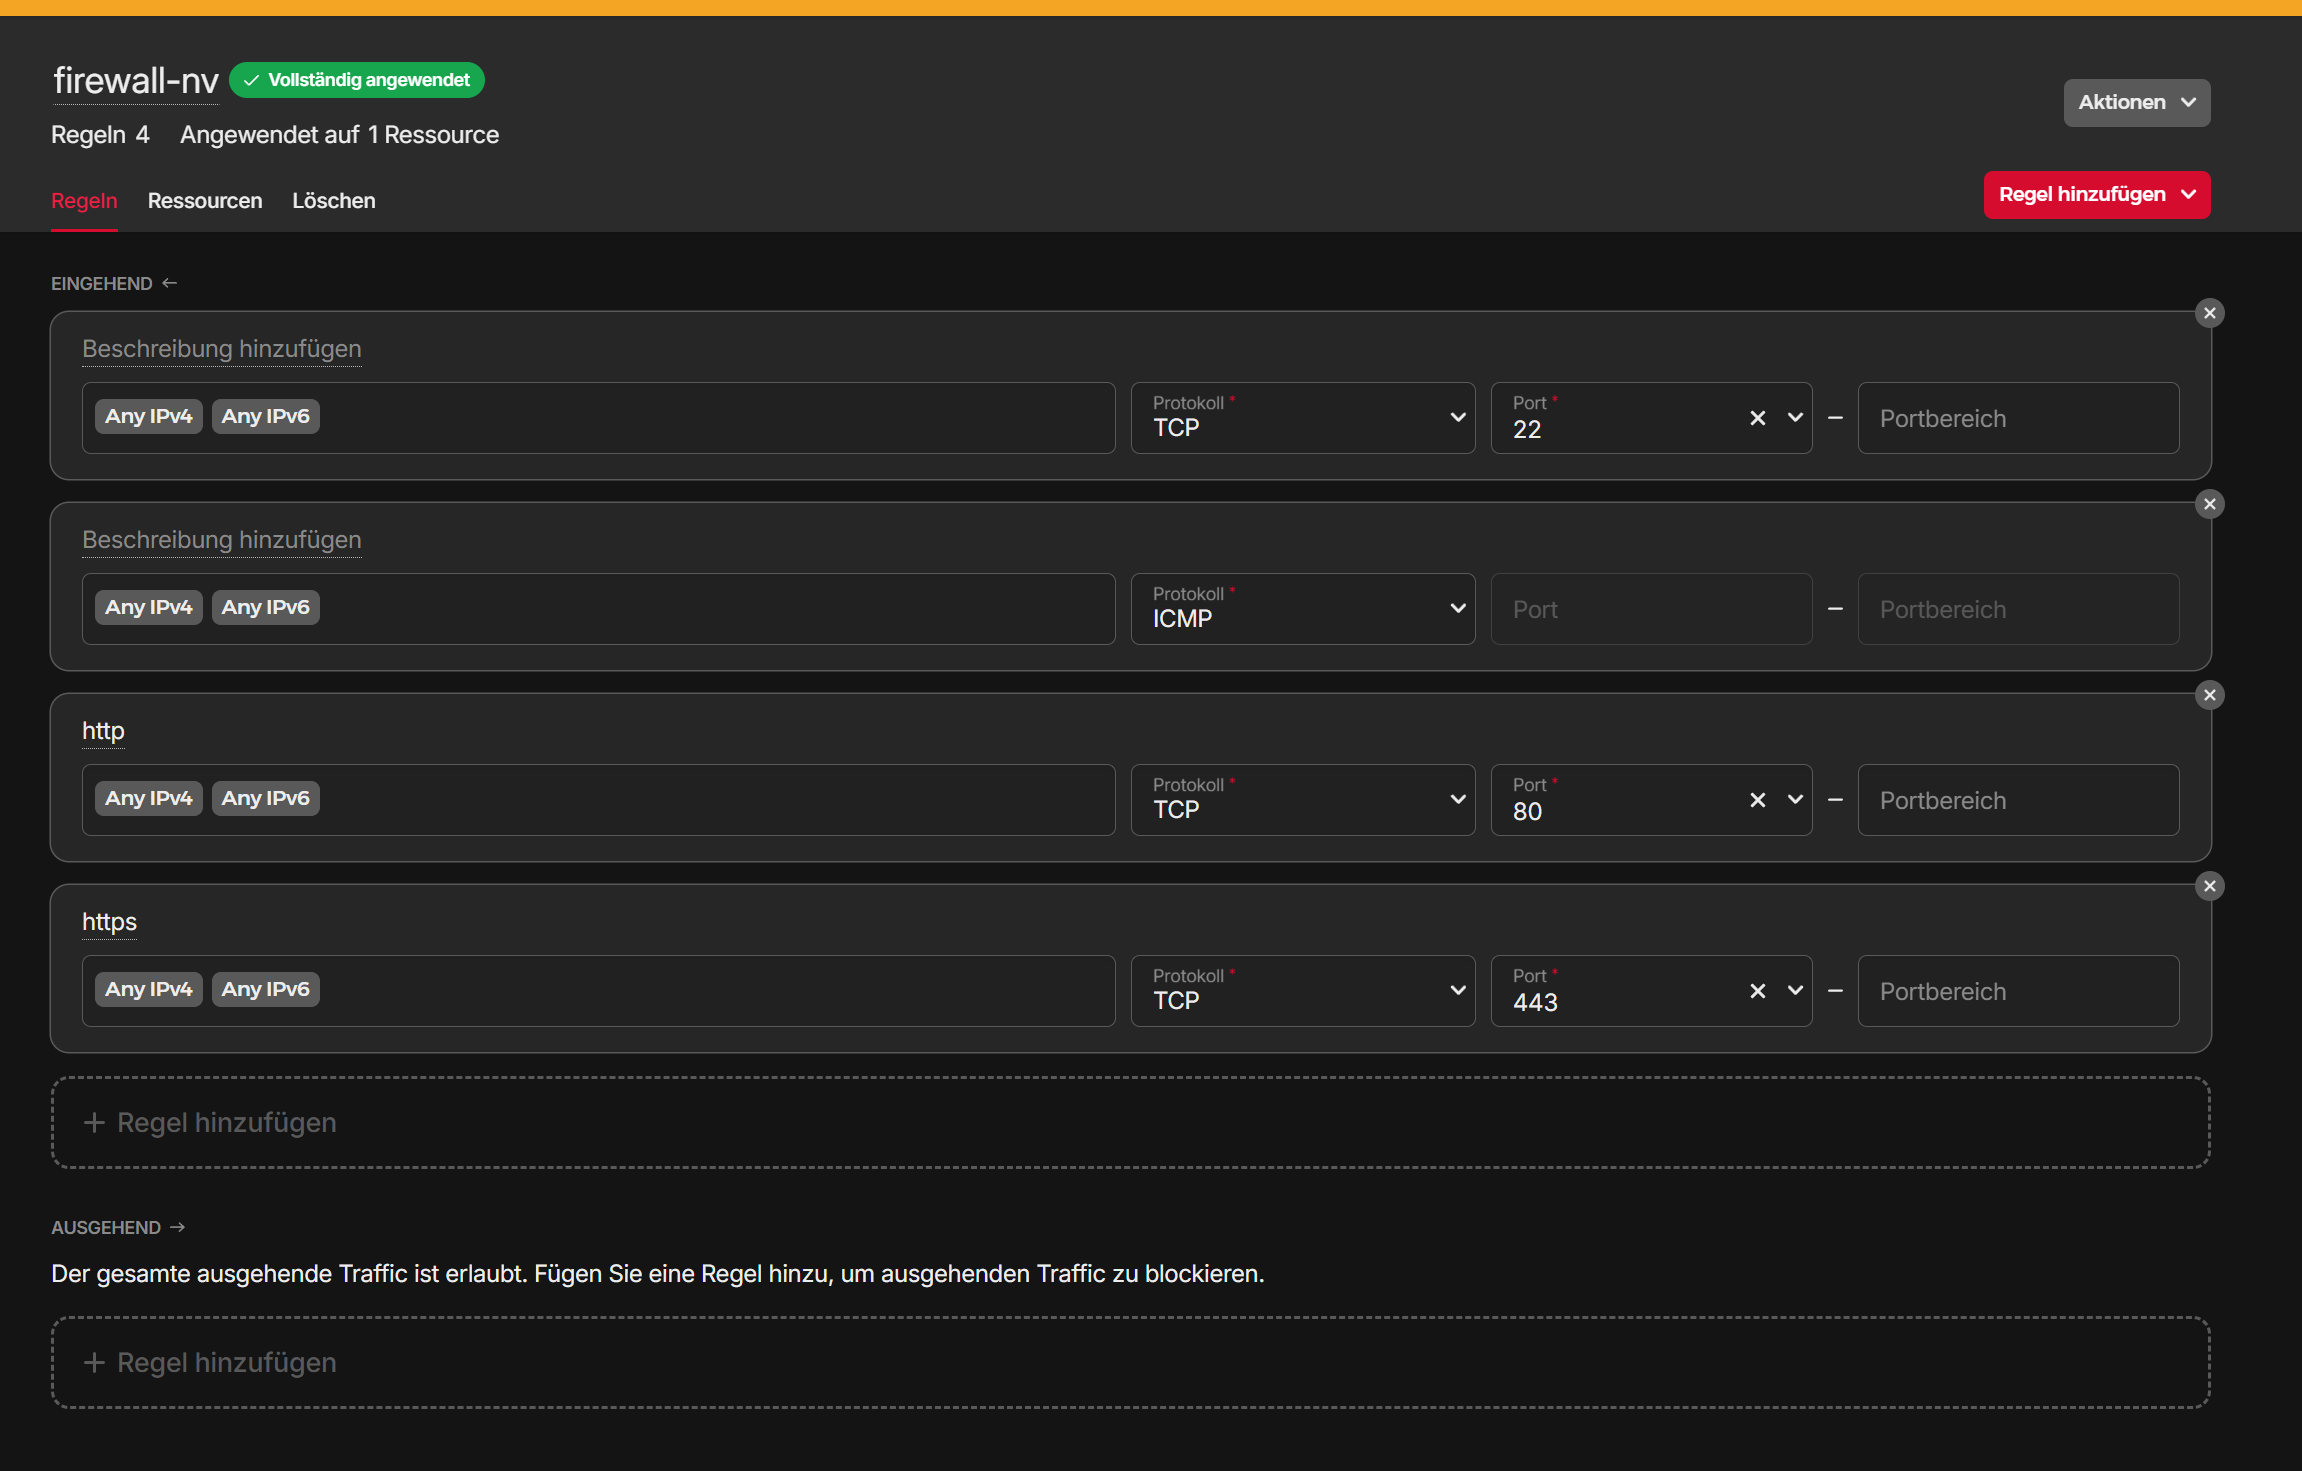
\includegraphics[width=0.95\linewidth]{images/firewall}
        \caption{Firewall in Hetzner}
        \label{fig:firewall}
    \end{figure}

    \subsubsection{DNS}
    In Cloudflare werden die DNS Records erstellt, damit die Domain auf die IP Adresse des Servers zeigt.
    \begin{figure}
        \centering
        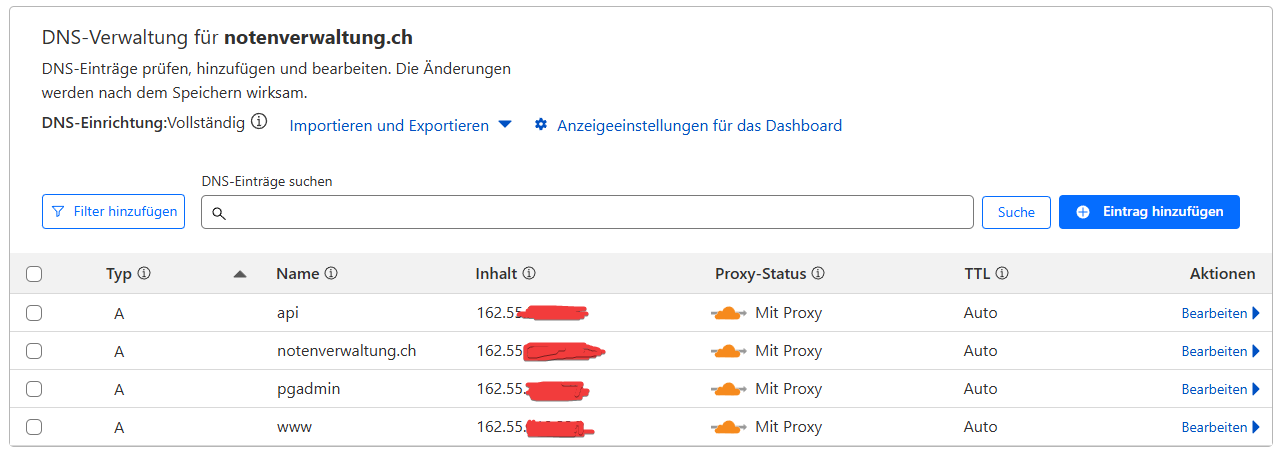
\includegraphics[width=0.95\linewidth]{images/dns}
        \caption{DNS Records in Cloudflare}
        \label{fig:dns}
    \end{figure}

    \subsection{Docker}

    \subsubsection{Installation}
    Docker wird mit den folgenden Befehlen installiert:
    \begin{lstlisting}[label={lst:InstallingDocker}]{language=bash}
# Add Docker's official GPG key:
sudo apt-get update
sudo apt-get install ca-certificates curl
sudo install -m 0755 -d /etc/apt/keyrings
sudo curl -fsSL https://download.docker.com/linux/ubuntu/gpg -o /etc/apt/keyrings/docker.asc
sudo chmod a+r /etc/apt/keyrings/docker.asc

# Add the repository to Apt sources:
echo \
  "deb [arch=$(dpkg --print-architecture) signed-by=/etc/apt/keyrings/docker.asc] https://download.docker.com/linux/ubuntu \
  $(. /etc/os-release && echo "${UBUNTU_CODENAME:-$VERSION_CODENAME}") stable" | \
  sudo tee /etc/apt/sources.list.d/docker.list > /dev/null
sudo apt-get update

sudo apt-get install docker-ce docker-ce-cli containerd.io docker-buildx-plugin docker-compose-plugin
sudo apt-get install docker-compose
    \end{lstlisting}
    Basierend auf der offiziellen Anleitung von Docker\cite{docker-ubuntu-install}.

    \subsection{Container}
    Damit die Container miteinander kommunizieren können, wird ein Docker Netzwerk erstellt.

    \subsubsection{Docker Netzwerk Anlegen}
    \begin{lstlisting}{language=bash}
    docker network create notenverwaltung_productive
    \end{lstlisting}

    \subsubsection{HTTPs}
    Für die HTTPS Verschlüsselung wird mit hilfe von Cloudflare ein kostenloses SSL Zertifikat erstellt.
    Dieses wird in der NGINX Konfiguration eingebunden.

    \subsubsection{Reverse Proxy}

    Der folgende Docker-Compose-Ausschnitt beschreibt den NGINX Reverse Proxy. Die wichtigsten Punkte sind:
    \begin{itemize}
        \item Volumes:
        \begin{itemize}
            \item \texttt{/mnt/volume-nbg1-1/data/proxy/conf.d/} wird nach \texttt{/etc/nginx/conf.d/} gemountet und enthält Proxy-Konfigurationen.
            \item \texttt{/mnt/volume-nbg1-1/data/proxy/www/} wird nach \texttt{/var/www/} gemountet für statische Dateien.
            \item \texttt{/mnt/volume-nbg1-1/data/proxy/ssl/} wird nach \texttt{/etc/ssl} gemountet und als read-only (\texttt{ro}) eingebunden für SSL-Zertifikate und Schlüssel.
        \end{itemize}
        \item Ports:
        \begin{itemize}
            \item \texttt{80:80} veröffentlicht HTTP nach ausen.
            \item \texttt{443:443} veröffentlicht HTTPS nach aussen.
        \end{itemize}
    \end{itemize}

    \lstinputlisting[language=yaml, label={lst:ComposeReverseProxy}, caption={docker-compose.yml für den Reverse Proxy}]{compose/reverse-proxy.yml}

    Die folgenden NGINX Server-Konfigurationen werden im Verzeichnis \texttt{conf.d} des Reverse Proxys abgelegt und definieren das Routing für die Domains.
    Jede Datei enthält jeweils eine Weiterleitung von HTTP auf HTTPS sowie einen verschlüsselten Server-Block, der Anfragen an den passenden
    internen Container im Docker-Netzwerk weiterleitet.

    Wichtige Punkte in allen Konfigurationen:
    \begin{itemize}
        \item \textbf{HTTP-zu-HTTPS-Weiterleitung}: Der Port-80-Server leitet alle Anfragen per 301 auf HTTPS um. Erhöht Sicherheit und SEO.
        \item \textbf{TLS-Konfiguration}: Die Zertifikate werden aus dem Volume unter \texttt{/etc/ssl} eingebunden (z. B. Cloudflare Origin-Zertifikate). HSTS ist aktiviert.
        \item \textbf{Proxy-Header}: \texttt{X-Forwarded-*}-Header und \texttt{Host} werden gesetzt, damit Backend und App die ursprünglichen Request-Informationen erhalten.
        \item \textbf{resolver 127.0.0.11}: Nutzt den internen Docker DNS-Resolver, sodass die Service-Namen (z. B. \texttt{api}, \texttt{frontend}, \texttt{pgadmin-prod}) aufgelöst werden.
        \item \textbf{client\_max\_body\_size}: Erlaubt grössere Uploads (z. B. Datei-Uploads der App).
    \end{itemize}

    \paragraph{notenverwaltung.ch (Frontend)} \texttt{frontend:80}

    \lstinputlisting[language=nginx, label={lst:NginxApex}, caption={NGINX vHost für notenverwaltung.ch}]{conf/notenverwaltung.apex.conf}

    \paragraph{api.notenverwaltung.ch (Backend API)}\texttt{api:8080}

    \lstinputlisting[language=nginx, label={lst:NginxApi}, caption={NGINX vHost für api.notenverwaltung.ch}]{conf/api.notenverwaltung.ch.conf}

    \paragraph{pgadmin.notenverwaltung.ch (Datenbank-Admin)} \texttt{pgadmin-prod:80}.

    \lstinputlisting[language=nginx, label={lst:NginxPgAdmin}, caption={NGINX vHost für pgadmin.notenverwaltung.ch}]{conf/pgadmin.notenverwaltung.ch.conf}

    \subsubsection{Datenbank \& PG Admin}

    Der folgende Docker-Compose-Ausschnitt beschreibt die PostgreSQL-Datenbank und die Verwaltungsoberfläche pgAdmin.
    \begin{itemize}
        \item Volumes:
        \begin{itemize}
            \item Postgres-Daten: \texttt{/mnt/volume-nbg1-1/data/db/postgres} wird nach \texttt{/var/lib/postgresql/data} gemountet.
            Persistiert alle Datenbank-Dateien dauerhaft.
            \item pgAdmin-Daten: \texttt{/mnt/volume-nbg1-1/data/db/pgadmin} wird nach \texttt{/var/lib/pgadmin} gemountet.
            Persistiert Benutzer- und Server-Konfigurationen von pgAdmin.
        \end{itemize}
        \item Environment:
        \begin{itemize}
            \item \texttt{POSTGRES\_PASSWORD}: Initiales Passwort für den Superuser \texttt{postgres}.
            \item \texttt{PGADMIN\_DEFAULT\_EMAIL} / \texttt{PGADMIN\_DEFAULT\_PASSWORD}: Zugangsdaten für das pgAdmin-Admin-Konto.
        \end{itemize}
        \item Netzwerke:
        \begin{itemize}
            \item Beide Dienste befinden sich im gemeinsamen Netzwerk \texttt{notenverwaltung\_productive}, sodass pgAdmin die Datenbank unter dem Hostnamen \texttt{postgres} erreichen kann.
            \item Externe Erreichbarkeit erfolgt optional ausschliesslich via Reverse Proxy (kein eigenes \texttt{ports}-Mapping in Compose nötig/gesetzt).
        \end{itemize}
        \item Ressourcen/Deploy:
        \begin{itemize}
            \item Für Postgres sind Speicher-Limits/Reservations gesetzt (512M/128M).
            \item \texttt{replicas: 1} für zustandsbehaftete Services.
        \end{itemize}
    \end{itemize}

    \lstinputlisting[language=yaml, label={lst:ComposeDb}, caption={docker-compose.yml für die Datenbank + PgAdmin}]{compose/db-pgadmin.yml}

    Für pgAdmin muss der Datenordner initial angelegt und die Berechtigungen korrekt gesetzt werden:
    \begin{lstlisting}{language=bash}
        sudo mkdir -p /mnt/volume-nbg1-1/data/db/pgadmin
        sudo chown -R 5050:5050 /mnt/volume-nbg1-1/data/db/pgadmin
        sudo chmod -R u+rwX /mnt/volume-nbg1-1/data/db/pgadmin
    \end{lstlisting}

    Der externe Zugriff auf pgAdmin sollte über den Reverse Proxy und per HTTPs erfolgen (z. B. \texttt{pgadmin.notenverwaltung.ch}).
    Direkte Portfreigaben am Container werden aus Sicherheitsgründen vermieden. Zusätzlich kann eine \texttt{servers.json}
    bzw. eine Konfigurationsdatei für vordefinierte Verbindungen verwendet werden. Diese könnte über ein weiteres Volume nach
    \texttt{/pgadmin4/servers.json} eingebunden werden. Details siehe offizielle pgAdmin-Dokumentation.

    \subsubsection{Notenverwaltung Applikation}

    Die folgende Compose-Definition beschreibt den produktiven Betrieb der Spring-Boot-API im gemeinsamen Docker-Netzwerk.
    \begin{itemize}
        \item Environment:
        \begin{itemize}
            \item \code{DB\_URL}: JDBC-URL zur PostgreSQL-Datenbank (Host \code{postgres} im gemeinsamen Netzwerk, Port \code{5432}).
            \item \code{DB\_USERNAME} / \code{DB\_PASSWORD}: Zugangsdaten des DB-Users mit den nötigen Berechtigungen.
            \item \code{JWT\_SECRET}: Geheimnis zur Signierung/Verifizierung der JWTs der Anwendung.
        \end{itemize}
        \item Netzwerk: Der Service ist ausschliesslich im Netzwerk \code{notenverwaltung\_productive} sichtbar und wird nur über den Reverse Proxy extern erreichbar gemacht.
        \item Ressourcen/Deploy: Ein Replikat (zustandslos), Rolling Update mit Wartezeit, sowie konservative Speicherlimits/Reservierungen (512M/128M).
    \end{itemize}

    \lstinputlisting[language=yaml, label={lst:ComposeApi}, caption={docker-compose.yml für den Spring Service}]{compose/api.yml}

    \subsubsection{Angular Frontend}

    Der folgende Compose-Ausschnitt beschreibt das statische Angular-Frontend, das in einem NGINX-Container ausgeliefert wird.
    Hinweise zur Konfiguration und zum Betrieb:
    \begin{itemize}
        \item Image: Enthält die gebauten statischen Dateien und eine NGINX-Konfiguration, die die App unter Port 80 bedient.
        \item Netzwerk: Läuft ausschliesslich im internen Netzwerk \code{notenverwaltung_productive}.
        Externe Erreichbarkeit erfolgt über den Reverse Proxy und den Hostnamen \code{notenverwaltung.ch}.
        \item Ressourcen/Deploy: Ein Replikat genügt; Rolling Update-Einstellungen analog zu den anderen Services; moderate Speicherlimits/Reservierungen (512M/128M).
        \item API-Endpoint: Die App ruft die Backend-API unter \code{https://api.notenverwaltung.ch} auf.
        Diese URL ist im Build bzw. der NGINX-Config hinterlegt.
    \end{itemize}

    \lstinputlisting[language=yaml, label={lst:ComposeFrontend}, caption={docker-compose.yml für das Angular Frontend}]{compose/frontend.yml}


    \section*{Quellen}
    \begin{thebibliography}{9}
        \bibitem{docker-ubuntu-install}
        Docker, Inc. "Install Docker Engine on Ubuntu — Install using the repository." Zugriff am 20.09.2025. Verfügbar unter: \url{https://docs.docker.com/engine/install/ubuntu/#install-using-the-repository}
    \end{thebibliography}
\end{document}